\chapter{Grammatik und Lehramt}
\label{sec:grammatikundlehramt}


\section{Grammatik in der Schule}
\label{sec:grammatikinderschule}

Diesem Kapitel kommt eine Sonderrolle zu.
Es wurde in der dritten Auflage vollständig neu hinzugefügt, und es behandelt nicht Phänomene der deutschen Grammatik, sondern Anwendungsfälle grammatischen Wissens.
Der Grund für das Hinzufügen eines solchen Kapitels ist primär, dass ein Großteil der Studierenden in sogenannten \textit{polyvalenten Studiengängen} (also solchen, die gleichzeitig Fachwissenschaft und Lehramtsstudium bedienen) an vielen Universitäten inzwischen das Lehramt als Berufsziel haben.
Diese Studierenden haben einen besonderen Anspruch darauf, dass die Lehrinhalte des Studiums zur späteren beruflichen Praxis, die im Gegensatz zu der von Fachstudierenden klar definiert ist, in Bezug gesetzt werden.
Die Frage nach der Rolle von Grammatik im Lehramtsstudium kann selbstverständlich nur auf Basis der Rolle der Grammatik im Schulunterricht diskutiert werden.
In diesem Abschnitt wird daher bündig ein Konzept von Grammatik in der Schule diskutiert.
In Abschnitt~\ref{sec:grammatikimlehramtsstudium} werden die Konsequenzen für das Lehramtsstudium gezogen und dieses Buch im Kontext des Lehramtsstudiums verortet.
Dieses Kapitel kann ohne Probleme für die weitere Lektüre übersprungen werden.%
\footnote{An den wenigen Stellen, an denen es für das weitere Verständnis nötig ist, wird gezielt auf einzelne Abschnitte dieses Kapitels zurückverwiesen, die dann ggf.\ gezielt gelesen werden können.}

\subsection{Bildungssprache und ihr Erwerb}
\label{sec:bildungsspracheundihrerwerb}

Wenn Kinder eingeschult werden, können sie bereits auf einem hohen Niveau sprechen, vollständige Sätze formulieren und diese erfolgreich in alltäglichen Kommunikationssituationen verwenden.%
\footnote{Wir beziehen uns hier der Einfachheit halber nur auf Kinder mit deutscher Erstsprache und ohne Lern- oder Kognitionsschwächen.
Insbesondere der steigende Anteil von Kindern mit mehrsprachigem und auch nicht-erstsprachlichem Hintergrund sollte aber in diesem Kontext insgesamt berücksichtigt werden.
Die zitierte und weiterführende Literatur enthält dazu viel Wichtiges.}
Es ist also nicht die primäre Aufgabe des Deutschunterrichts, Kindern elementare orale Kommunikationsfähigkeiten für Alltagssituationen zu vermitteln.
Hingegen ist es eine offensichtliche Aufgabe des Deutschunterrichts, die Schrift und die Schreibungen des Deutschen zu lehren.
Ein oft anzutreffender Irrglaube ist dabei, dass ungefähr mit der Primarstufe der Schrift- und Schriftspracherwerb abgeschlossen sei und es in diesem Bereich nur noch um das "`Ausmerzen"' verbleibender Schwächen gehe.
Es ist vielmehr davon auszugehen, dass der Orthographieerwerb sogar nach der Schulzeit (natürlich in Form eines sich sättigenden -- also stetig langsamer werdenden -- Prozesses) fortgeführt wird \citep[72]{Portmanntselikas2011}.
Der Erwerb der Schriftsprache muss aber vielmehr in einem größeren Rahmen betrachtet werden, nämlich dem des Erwerbs der \textit{Bildungssprache}.
Dieser Abschnitt widmet sich daher dem Bildungsspracherwerb.

Die Sprache, die vorliterate Kinder (die wir hier vereinfachend mit noch nicht eingeschulten Kindern gleichsetzen) sprechen, ist an bestimmte Situationen und Funktionen gebunden (Essen, Spielen, Aufräumen, Zeigen von verschiedenen Emotionen zur Stimulation einer Reaktion beim Gegenüber usw.) und wird weitgehend ohne systematische Instruktionen in diesen Situationen erlernt.
Mit der Einschulung und damit der Literalisierung verlangen wir von Kindern zunehmend auch die Fähigkeit, völlig andere Modi der Kommunikation zu bedienen.
Kinder sollen lernen, sowohl schriftlich als auch mündlich komplexe Sachverhalte darzustellen, Begriffe intensional (also nicht durch bloße Aufzählung von Beispielen) zu definieren, für oder gegen eine Sache zu argumentieren, in verschiedenen Situationen teilweise stark unterschiedliche angemessene sprachliche Mittel zu verwenden, die Standardsprache zu beherrschen und vieles dergleichen mehr.
Diese Fähigkeiten charakterisieren die \textit{Bildungssprache} (\zB \citealt{Feilke2012}).
Merkmale der Bildungssprachliche finden sich nun vor allem in Kontexten, denen vorliterate Kinder nicht ausgesetzt sind, \zB in schulischen Lernsituationen (wohlgemerkt in allen Fächern, nicht nur im Deutschunterricht) und im akademischen Bereich.
Darüberhinaus werden auch in Alltagssituationen von Erwachsenen ggf.\ ähnlich fortgeschrittene sprachliche Leistungen erwartet, zum Beispiel bei der Auseinandersetzung mit juristischen oder finanziellen Fragen oder der Lösung technischer Probleme \citep[5]{Feilke2012}.
Damit ist die Beherrschung der Bildungssprache "`gleichermaßen ein Bildungskapital, wie sie eine Hürde für das Verstehen sein kann"' \citep[11]{Feilke2012}.
Werden bildungssprachliche Kompetenzen nämlich nur unvollständig oder mangelhaft erworben, ist eine Teilhabe in vielen Bereichen der Gesellschaft nur eingeschränkt möglich.
Zugleich ist die bildungssprachliche Ausbildung auch für die schulische Karriere jenseits des Deutschunterrichts von besonderer Wichtigkeit, da die bildungssprachlichen Anforderungen in allen Fächern mit der Komplexität der Inhalte steigen.
Dementsprechend verlangen die Richtlinien der Kultusministerkonferenz auch gerne global, dass Lernende nach der Schulzeit in der Lage sein mögen, situationsangemessen und standardkonform zu sprechen und zu schreiben \citep[6]{Eisenberg2004}.

Dabei ist es nun richtig, dass sich die Schwerpunkte im Laufe der Erwerbskarriere von der Beherrschung basaler Orthographie mehr und mehr hin zu Fragen des Stils und der situationsangemessenen Schreibweise und Sprechweise verschieben \citep[77]{Portmanntselikas2011}, aber beide sind von Anfang bis Ende auf besondere Weise miteinander verknüpft.
Ein Großteil der Fachdidaktik des Deutschen und der didaktisch interessierten Linguistik des Deutschen versteht Standardsprache und Bildungssprache als untrennbar gekoppelt an die historische Entwicklung der Schrifttradition des Deutschen (\citealt[130--150]{Bredel2013}; auch \citealt{Nerius2007}).
Auf der kognitiven bzw.\ individuellen Seite werden bildungs- und standardsprachliche Kompetenzen bedingt und geformt durch den Erwerb der Schriftsprache.
In diese Richtung argumentieren zum Beispiel \citet[4,12,14,15]{Eisenberg2004}, \citet[71,78]{Portmanntselikas2011}, \citet[6]{Feilke2012}.
Für eine ausführlichere Betrachtung der Position von \citet{Bredel2013} siehe Abschnitt~\ref{sec:sprachbetrachtungundkonzeptederdeutschdidaktik}.

Der Schrift kommt eine besondere Rolle zu, weil sie bestimmte Charakteristika der Bildungssprache forciert.
Oben wurde betont, dass vorliterate Kinder Sprache vor allem situationsgebunden verwenden, und die erwähnten später erworbenen oder zu erwerbenden sprachlichen Kompetenzen wie Erläutern, Definieren, Argumentieren sind alle verbunden mit einer Loslösung der Sprache von der gegebenen Sprechsituation.
Es geht nicht mehr darum, in der aktuellen Situation mit unmittelbarer Wirkung sprachlich zu handeln, sondern zu größeren Zusammenhängen zu abstrahieren und allgemeine sowie komplexere Sachverhalte aufzugreifen und zueinander in Beziehung zu setzen.
Gleichzeitig geht damit eine Distanzierung von der eigenen sprechenden Person einher, weil die Perspektive der angesprochenen Personen (also das Verstehen der eigenen Äußerung) bei der Wahl sprachlicher Mittel berücksichtigt werden.
Anders gesagt:
Wir wollen verstanden werden und passen unsere Sprache daher den Zuhörenden und Lesenden an.
Dies alles wird mit dem Begriff der \textit{Dekontextualisierung} der Sprache erfasst.\index{Dekontextualisierung}%
\footnote{Eine einfache Form der Dekontextualisierung ist die berichtende Erzählung, zum Beispiel von Erlebtem.
Dabei werden Geschehnisse aus einem vergangenen -- also nicht dem gegenwärtigen -- Kontext wiedergegeben.
Freilich sind vorliterate Kinder dazu in der Lage.
Die Art, in der sie über erlebte Ereignisse berichten, unterscheidet sich aber erheblich von einem bildungssprachlich strukturierten Bericht, was die Gewichtung und Serialisierung der Teile der Erzählung angeht.
Wir alle kennen wahrscheinlich Erzählungen vorliterater Kinder, die aus einer Reihung von "`und dann \ldots"'-Konstruktionen bestehen, und denen zu folgen oft schwer ist, weil Ereignisse nicht nach ihrer Relevanz gewichtet wiedergegeben werden, und die damit insgesamt unter einem Mangel an Kohärenz leiden.
\citet{Bredel2013} enthält eine relevante Einführung in diesen Phänomenbereich jenseits solcher persönlichen episodischen Erfahrungen.}

Wichtig ist nun, dass die Schrift als Medium die Dekontextualisierung forciert.
Ein Schriftstück entsteht prototypischerweise ohne direkten Äußerungskontext und soll ohne einen solchen wirken.
Selbst dialogische Online-Kommunikation (vor allem Textnachrichten) muss ohne räumliche Nähe auskommen, und die schreibende Person muss für eine gelungene Kommunikation dabei in der Lage sein, zu verstehen und in ihren sprachlichen Äußerungen zu berücksichtigen, dass die angeschriebene Person nicht dasselbe sieht und hört wie sie selber.
Schriftsprache führt also automatisch zu einer Dekontextualisierung und fördert somit automatisch einen höheren Abstraktionsgrad des Gesagten.
Neben dieser engen Verbindung von wesentlichen Merkmalen der Bildungssprache und Schrift begünstigt Schrift die Herausbildung und die Reflexion über die Konformität zu einer wie auch immer gearteten Norm oder einem Standard und damit notwendigerweise eine Fokussierung auf formale Eigenschaften von Sprache \citep[41]{Bredel2013}.%
\footnote{Zur expliziten Reflexion über Sprache siehe auch Abschnitt~\ref{sec:sprachbetrachtungundkonzeptederdeutschdidaktik}.}
Einerseits nimmt es nicht wunder, dass die Herausbildung von Standards für ein bestimmtes Deutsch als allgemeine Verkehrssprache durch die weite Verbreitung von Schriftgut durch den Buchdruck und damit einen starken Zuwachs an literalisierten Personen Vorschub erhielt \citep[301--352]{Nerius2007}. 
Durch die Fixierung von Sprache in Form eines Schriftstücks und damit die Möglichkeit der Revision dieser Sprache sowie einer Reflexion über sie, die nicht durch die eigene Erinnerungsfähigkeit begrenzt wird, werden Überlegungen über angemessene und \textit{richtige} Sprache gefördert.
Auch in der individuellen Entwicklung wird daher die Frage nach der Richtigkeit von Sprache und der Norm vom geschriebenen Wort ausgehend auf orale Kommunikation erweitert (\zB \citealt[72]{Portmanntselikas2011}).
Immerhin sind die Gelegenheiten, zu denen es wirklich auf normnahe Sprache ankommt, in der oralen Kommunikation eher selten (\zB politische Ansprachen, Bewerbungsvorträge für Germanistikprofessuren), in der schriftlichen Kommunikation aber nahezu der Normalfall.

Die spezifischen \textit{Funktionen} der Schrift- und Bildungssprache gehen nun mit einem erweiterten und komplexeren Inventar von \textit{formalen Mitteln} bzw.\ mit einer anspruchsvolleren Verwendung der existierenden formalen Mittel einher.\index{Form und Funktion}
\citet[8--9]{Feilke2012} gibt eine beispielhafte Liste von anspruchsvollen formalen Mitteln, die für Bildungssprache charakteristisch sind, und die er bestimmten funktionalen Bereichen zuordnet.
Zum Bereich des \textit{Explizierens}, also dem Verständlichmachen von komplexen Sachverhalten, zählt er komplexe Adverbiale, Attribute und explizite Satzverbindung (\zB kausal oder adversativ).
Für den Bereich des \textit{Diskutierens}, also der Abwägung von Sachverhalten bezüglich ihres Wahrheitsgehalts, listet er beispielhaft den Gebrauch von Modalverben, Konjunktionen und konzessiven Konstruktionen.%
\footnote{Die beiden anderen von \citet[8--9]{Feilke2012} diskutierten Bereiche sind die des \textit{Verdichtens} und \textit{Verallgemeinerns}.}
Diese Mittel werden in der situationsgebundenen Alltagssprache erheblich seltener gebraucht (siehe auch \citealt[82--83]{Portmanntselikas2011}) und mit Beginn der Literalisierung erst -- zusammen mit den zugehörigen anderen kognitiven Fähigkeiten, die auf der inhaltlichen Seite erforderlich sind -- langsam ausgebildet.
Es ist also ein Irrtum, zu glauben, dass Kinder in der Schule einfach nur eine ihnen bereits bekannte Sprache schreiben lernen.
Vielmehr wird ihre gesamte Grammatik umgebaut, erweitert, um neue Register bereichert und in ihrem Stil verändert \citep[4,12--15]{Eisenberg2004}.
Zudem findet eine Ausrichtung auf die Norm und ein Bewusstmachen von Sprache statt, das vorher nicht existiert (siehe Abschnitt~\ref{sec:sprachbetrachtungundkonzeptederdeutschdidaktik}).

Damit ist also die Aufgabe des Deutschunterrichts \textit{für die gesamte Schulzeit} und nicht etwa nur für die Primarstufe definiert.
Die Aufgabe könnte nicht größer und verantwortungsvoller sein.
\citet[7]{Eisenberg2013c} spricht davon, dass den Lehrenden die Sprache der Lernenden "`anvertraut"' werde.
Der Umbau der Sprache von Schulkindern betrifft, wie oben argumentiert wurde, sprachliche Formen und Funktionen.
Da die Grammatik die Disziplin ist, die sich mit den sprachlichen Formen beschäftigt, ist die Frage nach dem Zweck von grammatischem Wissen für angehende Lehrpersonen im Fach Deutsch eigentlich bereits beantwortet.
Es wird aber gerne die Frage gestellt, welches Grammatikwissen das richtige sei, und ob die Grammatik nicht der Form an sich einen zu hohen Stellenwert beimesse.
In Abschnitt~\ref{sec:sprachbetrachtungundkonzeptederdeutschdidaktik} werden daher kurz didaktische Konzepte für den Deutschunterricht und der Systembegriff der Grammatik diskutiert.


\subsection{Sprachbetrachtung und Konzepte der Deutschdidaktik}
\label{sec:sprachbetrachtungundkonzeptederdeutschdidaktik}

Eins der Ziele dieses Kapitels ist es, für die Existenzberechtigung der systematischen Grammatik in der Schule und dem Germanistikstudium zu argumentieren.
Es mag auf Verwunderung stoßen, dass sich die Grammatik überhaupt zu rechtfertigen versucht.
Dies hat damit zu tun, wie sich das Verhältnis zwischen (1) der Linguistik des Deutschen, (2) der Fachdidaktik des Fachs Deutsch und (3) dem Lehrpersonal des Schulfachs Deutsch entwickelt hat.
Eine umfassende Betrachtung der Geschichte der Deutschdidaktik gehört nicht hierher, aber die wesentlichen Linien, die zur heutigen Situation geführt haben, sind recht einfach.%
\footnote{Ich folge wie im Rest dieses Abschnitts der ausführlichen Einführung aus \citet{Bredel2013} (hier besonders Abschnitt~3.1).
Bei Bredel finden sich zahlreiche zusätzliche Referenzen.
Siehe auch \citet{Gornik2003}.}

Der {traditionelle Grammatikunterricht} der ersten Hälfte des zwanzigsten Jahrhunderts ist ein rein an der Form orientierter deklarativer Benennungsunterricht.
Aus der Lateingrammatik entlehnte Kategorien werden auf das Deutsche übertragen, und die Leistung der Lernenden besteht darin, Wortarten, Nebensatztypen, grammatische Funktionen usw.\ in Sätzen zu identifizieren und zu benennen.
Dass dieser Ansatz beim Erlernen der Bildungssprache nicht sonderlich hilfreich sein dürfte, erscheint heute offensichtlich.%
\footnote{Umso erstaunlicher ist es, dass immer noch traditionell Grammatik unterrichtet wird, worauf im weiteren noch eingegangen wird.}
Mit den späten sechziger Jahren des zwanzigsten Jahrhunderts kommt allerdings im Rahmen eines generellen Zweifels an traditionellen Lehrmethoden und im Sinne einer Sprachkritik Bewegung in die Angelegenheit, und es setzte eine konstante Diskussion in mehreren Wellen (bzw.\ \textit{Wenden}) ein.

Nach dem gescheiterten Versuch der Linguistik, in den siebziger Jahren die sogennante \textit{generative Transformationsgrammatik} (ein abstrakt-algebraisches und nach zehn Jahren bereits überholtes theoretisches Syntaxmodell) für den Schulunterricht nutzbar zu machen, kam es zu einer anti-formalen und anti-systematischen \textit{kommunikativen Wende}.
Im \textit{situativen Sprachunterricht} der späten siebziger Jahre (\citealt[229--232]{Bredel2013}; \citealt{BoettcherSitta1978}) wurden grammatische Eigenschaften von sprachlichen Äußerungen nur als Teil der situativ-kommunikativen Funktion von Sprache betrachtet.
Die Vermittlung sollte allein in rein situativen Lehranlässen und nicht abstrakt-systematisch erfolgen.
Das Hauptproblem dieses Ansatzes ist die Unmöglichkeit, durch rein situative Vermittlung (allein schon durch die Begrenztheit der zeitlichen Ressourcen in der Schule) ein echtes systematisches Wissen aufzubauen.
Darüberhinaus verlangt diese Methode von den Lehrpersonen ein sehr hohes Maß an sprachsystematischer und sprachdidaktischer Kompetenz.

Der \textit{funktionale Grammatikunterricht} der achtziger Jahre und darüberhinaus (\citealt[233--239]{Bredel2013}; \citealt{Koeller1997}) strebt durchaus eine systematische Betrachtung an.
Es wird auf bestimmte Erkenntnisprozesse bei Lernenden gesetzt.
Sie sollen Funktionen von sprachlichen Äußerungen erkennen und lernen, sie kritisch zu hinterfragen sowie produktiv mit ihnen umzugehen usw.
Der Fokus liegt hier allerdings ausschließlich auf systemexternen Funktionen von Sprache (siehe Abschnitt~\ref{sec:formundfunktionindergrammatik}), und die interne Systematik der Grammatik bleibt außen vor.
Während also durchaus systematisch und teilweise induktiv vorgegangen wird, wird nicht im eigentlichen Sinn Grammatik (also eine Formbetrachtung) angestrebt.

Für das hier vorgelegte Buch ist die \textit{Grammatik-Werkstatt} der neunziger Jahre (\citealt{EisenbergMenzel1995}; \citealt{Menzel2017}; \citealt[Abschnitt~3.2.4]{Bredel2013}) mit Abstand der einflussreichste Vorschlag einer Methode für den Deutschunterricht.\index{Grammatik-Werkstatt}
Sie setzt auf systematische Grammatik, aber entgegen dem traditionellen Grammatikunterricht basiert sie auf induktiven Erkenntnisprozessen anhand von gezielt ausgewähltem sprachlichen Material.
Durch ein gesteuertes Arbeiten (bzw.\ ein Spiel) mit Formen und Formenreihen erfassen die Lernenden Muster und Regularitäten.
Sind diese Muster und Regularitäten erkannt, können sie zu Funktionen in Beziehung gesetzt werden.
Das Verfahren ist induktiv, setzt also auf Erkenntnisse auf Basis der Betrachtung von sprachlichem Material, nicht etwa auf die Vermittlung eines gegebenen oder gar theoretischen Wissens ex cathedra.
Durch diese Methode sollen die Ergebnisse besser im Gedächtnis verankert werden.
Zudem soll die Fähigkeit erworben werden, auch über den Unterrichtsstoff hinaus grammatisch zu arbeiten.
Vor allem ist zu bemerken, dass die in der Grammatik-Werkstatt vertretene Methode der grundlegenden Methode der traditionellen Linguistik entspricht \citep[239]{Bredel2013}.
Natürlich setzt das Spiel mit Formen und Formenreihen eine bestehende Intuition über Sprache bei den Lernenden voraus und ist damit vor allem an die Erstsprache gebunden.
Die vorhandene Intuition soll aber weiter geschult und systematisiert werden \citep[241]{Bredel2013}.
Auf diesen Ansatz kommen wir später noch zurück.

Bei alledem ist aber zunächst ernüchternd festzustellen, dass neue Methoden den Schulunterricht gar nicht oder nur bruchstückhaft erreichen.%
\footnote{Erst kürzlich wurde mir gegenüber in persönlicher Kommunikation aus linguistischen Kreisen vehement argumentiert, dass die Linguistik viel zur Weiterentwicklung der realen schulischen Deutschdidaktik beigetragen hätte.
Insbesondere die Lehramtsinitiative der Deutschen Gesellschaft für Sprachwissenschaft wurde in diesem Zusammenhang erwähnt.
Es muss betont werden, dass die Lehramtsinitiative eine der wenigen langjährigen Initiativen ist, die den Dialog zwischen der germanistischen Linguistik und Lehrpersonen aufrechterhalten.
Allerdings wird in der Literatur zur Didaktik des Deutschen immer wieder betont, dass die Schulwirklichkeit im Prinzip auf dem Stand des traditionellen Grammatikunterrichts stehengeblieben ist (\zB \citealt[211]{Steets2003} und dort zitiert \citealt[143]{SteinigHuneke2002}; \citealt[243,257]{Bredel2013}; \citealt[2]{KoepckeZiegler2013}).}
Offiziell geben die Richtlinien des Bundes und der Länder -- auch in den neueren "`kompetenzorientierten"' Formulierungen -- wenig Konkretes vor \citep[250--255]{Bredel2013}.
Statt der oben beschriebenen aufwändig entwickelten Konzepte hat vor allem die \textit{Terminiliste} der Kultusministerkonferenz Berühmtheit erlangt \citep[244--249]{Bredel2013}.
In dieser Liste werden zahlreiche (und in ihrer Auswahl umstrittene) grammatische Begriffe, die Lernenden nach ihrer schulischen Laufbahn bekannt sein sollen, schlicht und einfach aufgelistet.
Diese liefert allerdings keine Definitionen und keine Methoden der Vermittlung, ist also eher ein Mittel, das in der Praxis den traditionellen Grammatikunterricht fördert.
Zudem kennen selbst Lehrpersonen diese Liste nur zu einem geringen Prozentsatz \citep{Haecker2009}.

Die Ideen der letzten fünfzig Jahre für den schulischen Grammatikunterricht waren also von einem Richtungsstreit geprägt.
Soll der Grammatikunterricht formal oder funktional ausgerichtet sein?
Soll er induktiv vorgehen -- also Erkenntnisprozesse auf Basis von sprachlichen Daten fördern -- oder deduktiv sein -- also ein feststehendes Wissen vermitteln?
Mit alldem verbunden ist auch die Frage, ob es überhaupt einen expliziten Grammatikunterricht geben muss.
Wir argumentieren hier, dass die Fähigkeit zur \textit{Sprachbetrachtung} wesentlich für bildungssprachliche Kommunikation und damit Teil unserer Sprachkultur ist.\index{Sprachbetrachtung}

Allen Konzepten des schulischen Grammatikunterrichts, die wir oben in diesem Abschnitt besprochen haben, ist mehr oder weniger gemein, dass sie die Lernenden in die Lage versetzen sollen, über Sprache explizit nachzudenken, um dadurch gezielt Entscheidungen über ihren eigenen Sprachgebrauch fällen zu können.
Dies steht wiederum im Dienst der Beherrschung der Schrift- und Bildungssprache (s.\ Abschnitt~\ref{sec:bildungsspracheundihrerwerb}).
\citet[14]{Bredel2013} stellt richtig fest, dass zum elementaren Beherrschen einer Sprache keine Reflexion über diese Sprache selber erforderlich ist.
Sprachbetrachtung ist aber eine alltägliche Tätigkeit, \zB wenn wir nach den richtigen Wörtern suchen, wenn wir Fragen der Orthographie und Interpunktion nachgehen, wenn wir die Ausdrucksweise von einem Gegenüber im Diskurs bewerten \citep[22]{Bredel2013}.
Das Gleiche gilt, wenn wir \zB Formulierungen in Texten optimieren oder Schreibvarianten ausprobieren \citep[23]{Bredel2013}.
In Anlehnung an \citet{Clark1978} spricht \citet[35]{Bredel2013} auch von Sprachbetrachtungsaktivitäten wie dem sprachlichen Einstellen auf zuhörende Personen, dem Kommentieren und Korrigieren von Äußerungen anderer, der expliziten Definition sprachlicher Begriffe, der Erklärung von Bedeutungen und Grammatikalität.
Diese Dinge sind in der Tat sprachlicher Alltag und eine Folge dessen, dass wir unsere Kultur stark am geschriebenen Wort -- und der vom geschriebenen Wort ausgehenden Bildungssprache -- ausgerichtet haben.%
\footnote{Die Sprachwissenschaft von Sprachen wie dem Deutschen ist im übrigen selber schriftorientiert.
Auch wenn manchmal in der Linguistik das \textit{Primat der gesprochenen Sprache} beschworen wird (dazu mehr in Abschnitt~\ref{sec:graphematikalsteildergrammatik}), attestiert \citet[40]{Bredel2013} dies korrekt.}

Zur Bildungssprache gehört also die Fähigkeit zur expliziten Sprachbetrachtung.
Inwiefern durch sprachbetrachtenden Schulunterricht allerdings direkt das sprachliche Handeln von Lernenden beeinflusst werden kann, ist nicht geklärt (\citealt[73,75--79,80]{Portmanntselikas2011}; \citealt[94]{Bredel2013}; \citealt[8]{Eisenberg2013c}; \citealt[2]{KoepckeZiegler2013}).
Wir wissen also nicht, ob es zum Beispiel Kindern in der Primarstufe hilft, ihre eigenen sprachlichen Fähigkeiten zu verbessern, wenn wir sie in Grammatik unterrichten.
Die Grammatik in der Schule aufzugeben, wird aber kaum jemand wagen, denn insbesondere der Erwerb der Orthographie und Interpunktion erfordert das Explizieren von grammatischen Sachverhalten \citep[9--10]{Eisenberg2013c}.
Natürlich könnte man sich darauf verlassen, dass Kinder, die freiwillig viel lesen, die Orthographie und Interpunktion einwandfrei auch ohne langjährige Instruktion lernen.
Aber niemand würde erwägen, Kinder nach der Einführung der Buchstaben nicht weiter im Schreiben zu unterrichten und darauf zu hoffen, dass sie freiwillig qualitativ und quantitativ ausreichende Lektüre konsumieren.
Ganz unabhängig von der nur unvollständig erforschten Wirkung des frühen Grammatikunterrichts auf den Bildungsspracherwerb ist Grammatikunterricht insgesamt aber eben auch eine langfristige Ausbildung zur Sprachbetrachtung, und diese ist Bestandteil unseres sprachlichen Alltags.

Im nächsten Abschnitt wird bezüglich der vorgeschlagenen Konzepte für den Grammatikunterricht Stellung bezogen.


\subsection{System und Funktion im Grammatikunterricht}
\label{sec:systemundfunktionimgrammatikunterricht}

Wir haben gezeigt, dass im Sinn der Förderung des Schrift- und Bildungsspracherwerbs schulischer Deutschunterricht zur Sprachbetrachtung anleiten soll.
Die oben beschriebenen didaktischen Modelle des Grammatikunterrichts (traditionell, situativ, funktional, Grammatik-Werkstatt) unterscheiden sich vor allem auf drei Achsen (siehe auch \citealt[8--9]{Menzel2017}):
erstens \textit{deduktiv vs.\ induktiv}, zweitens \textit{systematisch vs.\ nicht-systematisch}, drittens \textit{funktional vs.\ nicht-funktional}.%
\footnote{Hier wird bewusst nicht \textit{funktional} gegen \textit{formal} gestellt.}

Der traditionelle Unterricht ist deduktiv, das heißt er vermittelt ein einmal festgelegtes Wissen, und sprachliches Material wird zu diesem Wissen in Beziehung gesetzt, also in den Begriffen und Kategorien der traditionellen Grammatik analysiert.
Alle anderen Ansätze sind ganz oder teilweise induktiv, sie setzen also auf Erkenntnisprozesse bei den Lernenden, die auf gegebenem Material aufbauen.
Es scheint also in der neueren Didaktik ein Konsens darüber zu bestehen, dass Lernenden in der Schule nicht einfach ein deklaratives Wissen vorgesetzt werden soll.
Der traditionelle Grammatikunterricht kann daher als disqualifiziert gelten.

Bezüglich der Unterscheidung von systematischem und nicht-systematischem Unterricht steht die Grammatik-Werkstatt von den verbleibenden Ansätzen alleine auf der Seite des grammatischen Systems.%
\footnote{Das in \citet{Bredel2013} vorgeschlagene Konzept ist nicht identisch zur Grammatik-Werkstatt, setzt aber wie diese auf einen systematischen Zugang.}
Der situative Sprachunterricht setzt auf in konkreten Situationen erworbenes Inselwissen, der funktionale geht von der Funktion aus und vermittelt eher pragmatisches Wissen als systematische Grammatik.

An dieser Stelle müssen einige wesentliche Punkte berücksichtigt werden.
Erstens wurde in Kapitel~\ref{sec:grammatik} bereits argumentiert, dass das System der Grammatik ein Eigenleben (jenseits der kommunikativen Funktion sprachlicher Zeichen) hat.
Zweitens zeigt bereits Kapitel~\ref{sec:grundbegriffedergrammatik}, wie komplex dieses System eigentlich ist, und wie trotzdem auf Basis von sprachlichem Material Begriffe wie Rektion und Valenz induktiv erarbeitet werden können.
Drittens wissen wir auch aus Kapitel~\ref{sec:grammatik}, dass die Norm (also zum Beispiel das Standarddeutsche) nur schwer greifbar ist, dass nicht jeder sprachliche Zweifelsfall überhaupt normativ geregelt ist, und dass Sprache (selbst im Standard oder in der Nähe des Standards) starker Variation zwischen Regionen, persönlichen Stilen, situativen Registern usw.\ unterliegt.
Viertens geht Schulunterricht aber nicht ohne Norm, denn Eltern würden zurecht widersprechen, wenn Lehrpersonen ihren Kindern "`rein deskriptive Sprachbetrachtung"' beibrächten.
Fünftens muss festgestellt werden, dass die Zeit, die dem Deutschunterricht -- und insbesondere der Sprachbetrachtung und der Grammatik -- in der Schule eingeräumt wird, angesichts der zu bewältigenden Aufgabe äußerst knapp ist.

Nimmt man diese Punkte zusammen, kommt man um einen Unterricht nicht herum, der das grammatische System als Ganzes im Blick hat.
In der Kürze der Zeit und angesichts der Komplexität des Systems wird ein kleinteiliger rein kommunikativ-funktional ausgerichteter Unterricht die Lernenden nicht in den Stand versetzen, souverän normkonforme bildungssprachliche grammatische Entscheidungen zu treffen.
Sprachbetrachtung hilft, den Standard als eine von vielen Varietäten zu verstehen und von diesen zu unterscheiden.
Gleichzeitig ist sie der Schlüssel zum Verständnis der Variation \textit{innerhalb} des Standards in Form von Stil- und Registerspezifik.
Das funktioniert aber nur, wenn die verschiedenen Varietäten (aller Art) als System begriffen werden, das auf die zugrundeliegenden Möglichkeiten des grammatischen Systems aufbaut (\citealt[10--11]{Eisenberg2004}; siehe auch \citealt[10]{Menzel2017}).
Gegen ausufernden Formenpluralismus (rein deskriptive Grammatik) auf der einen Seite und Regulierungswut (also den Glauben an die Einheitslösung, die irgendwo in einer Normgrammatik gesucht wird) auf der anderen Seite stellt \citet[8--9]{Eisenberg2004} die Ausbildung zur Fähigkeit, sprachliche Formen in das System einzuordnen und die Bedeutungs- und Gebrauchsunterschiede im Zweifelsfall selber analysieren zu können.%
\footnote{Auch \citet[80--83]{Portmanntselikas2011} argumentiert, dass ein Sprachunterricht, der eine systematische und nicht bloß inselhaft-episodische Wirkung haben soll, auf begrifflich fassbare Regularitäten zurückgreifen muss.
Grammatisches Wissen, das nur exemplarisch und damit inselhaft bzw.\ nicht systematisch eingeführt wird, reicht nicht aus, weil die Reichweite der entsprechenden Regularität nicht notwendigerweise erkannt wird.}

Mit der Forderung nach einem induktiven, systematischen und funktionalen Grammatikunterricht im Rahmen der Ausbildung in Schrift- und Bildungssprache beenden wir diese kurzen Überlegungen zum schulischen Spracherwerb.
In Abschnitt~\ref{sec:grammatikimlehramtsstudium} werden die entsprechenden Schlussfolgerungen für das Lehramtsstudium gezogen.

\begin{Vertiefung}{Vor der Fähigkeit zur Sprachbetrachtung}
\label{vert:faehigkeitzursprachbetrachtung}

\noindent Insbesondere angehende Lehrperson in der Grundschule kommen um eine Beschäftigung mit den Fähigkeiten vorliterater Kinder nicht herum.
\citet[52--56]{Bredel2013} gibt einen Überblick über klassische Experimente, die gezeigt haben, dass vorliterate Kinder grundlegend andere Konzepte von Sprachbetrachtung haben.
Insbesondere ist die Orientierung an der sprachlichen Form, zu der Erwachsene tendieren, kaum ausgeprägt.
Hier können nur einige Beispiele kurz angesprochen werden, die Lektüre von \citet{Bredel2013} und \citet[71--134]{BredelEa2017} liefert die Details, die insbesondere für Lehrende im primarstuflichen Deutschunterricht unverzichtbares Wissen darstellen.

Vorliterate Kinder, die zur Sprachbetrachtung aufgefordert werden reflektieren in der Regel über den \textit{Inhalt} der Wörter oder Sätze, nicht über deren Form.
Zum Beispiel werden kurze Wörter, die große Gegenstände bezeichnen (\zB \textit{Haus}), gegenüber langen Wörtern, die kleine Gegenstände bezeichnen (\textit{Streichholzschächtelchen}), als die längeren klassifiziert \citep{Bosch1984}.
Das Wort als vom bezeichneten Gegenstand unabhängige Einheit wird also nicht erkannt.

Zur sprachlichen Assoziation aufgefordert assoziieren vorliterate Kinder zu Substantiven eher Situationen und Ereignisse, also \zB \textit{schlafen gehen} als Assoziation zu dem Substantiv \textit{Bett}, während Erwachsene tendentiell ähnliche Gegenstände benennen und in der grammatischen Kategorie (hier: Substantive) bleiben \citep{Entwistle1966}.
Solche Kinder analysieren Wörter also nicht formal und trennen sie damit von ihrer Bedeutung, sondern sehen sie holistisch.
In anderen Experimenten, die dies sehr deutlich machen, wurden vorliterate Kinder dazu aufgefordert, zu erklären, warum Wörter die Form haben, die sie haben.
Im Fall des Worts \textit{Geburtstag} werden \zB von einer Mehrheit Erklärungen gegeben, die sich nicht auf die Kompositionsstruktur beziehen.
Als Benennungsmotiv werden Dinge benannt wie der Erhalt von Geschenken oder Kuchen.
Es werden also die wichtigen inhaltlichen Verknüpfungen mit dem Wort zur Definition verwendet, nicht die Form kompositional analysiert \citep{Berko1974}.

In Experimenten zur Satzsyntax wurden vorliterate Kinder dazu aufgefordert, die Anzahl der Wörter in Sätzen zu nennen.
Je nach Experiment wurden Sätze als ein Wort gezählt, nur die Inhaltswörter (vor allem Substantive) gezählt, oder in den Sätzen vorkommende Zahlwörter wurden als Anzahl der Wörter angegeben \citep{PapandropoulouSinclair1974}.
Auf der anderen Seite gelang es Kindern gleichen Alters erfolgreich, die \textit{letzten} Wörter von Sätzen zu benennen \citep{Karmilofsmith1996}.
Die mentale Grammatik der Kinder funktioniert also wahrscheinlich durchaus mit einem Konzept von Wörtern, aber der explizite reflektierende Zugriff erfolgt mit erheblichen Einschränkungen.
In jedem Fall ist die Formorientierung kein natürlicher Reifungsprozess, sondern eine Rekonzeptualisierung des grammatischen Systems auf Basis des Schrifterwerbs \citep[56]{Bredel2013}.

\end{Vertiefung}

\Zusammenfassung{%
Neben der Vermittlung der Schrift und der Schriftsprache ist die Vermittlung der Standard- und Bildungssprache die wichtigste Aufgabe des schulischen Deutschunterrichts.
Die Bildungssprache ist durch eine starke Dekontextualisierung bestimmt, die im schriftlichen Modus geradezu erzwungen wird.
Der Deutschunterricht vermittelt bildungssprachliche Kompetenzen in Form von expliziter Sprachbetrachtung (also von Nachdenken über Sprache), die langfristig zu primärsprachlichem Handeln führen soll.
Das Ziel, dass kompetent Sprechende (durch die Auswirkungen aktiver Sprachbetrachtung) stets diejenige sprachliche Form wählen, die zur intendierten kommunikativen Funktion passt, kann nicht erreicht werden, wenn das grammatische System (das System der Formen) nicht verstanden wird.
Schulunterricht in Grammatik muss also systematisch vorgehen.
Methodisch bauen wir auf einen induktiven Unterricht, der bei den Lernenden Erkenntnisprozesse auf Basis gezielt zusammengestellten sprachlichen Materials in Gang setzt.
Dadurch wird die Fähigkeit geschult, selber (auch jenseits von Gelerntem) grammatische Sachverhalte zu durchschauen.
}


\section{Grammatik im Lehramtsstudium}
\label{sec:grammatikimlehramtsstudium}

\subsection{Aufgaben der Linguistik im Lehramtsstudium}
\label{sec:aufgabenderlinguistikimlehramtsstudium}

Die Aufgaben der Linguistik im Rahmen der Lehramtsausbildung müssen vor allem vor dem Hintergrund dessen formuliert werden, was Lehrpersonen in ihrem späteren Arbeitsalltag im Rahmen des Unterrichts in Sprachbetrachtung und Bildungssprache zu leisten haben.
\citet[7]{Eisenberg2013c} benennt die wichtigsten Aufgaben, nämlich das Erkennen sprachlicher Defizite der Lernenden, die Identifikation der dialektalen Prägung der Lernenden (da diese oft die stärkste erstsprachliche Hürde für bildungssprachliches Sprechen darstellt), sowie die Berücksichtigung von Interferenzen mit anderen Erstsprachen (insbesondere bei nicht erstsprachlichen Lernenden).
Dies erfordert laut Eisenberg, dass Lehrende sich auf die Sprache der Lernenden einlassen und sie im Sinn eines analytischen Verständnisses durchschauen können.
Selbstverständlich kann dies nicht ohne ein vertieftes Wissen über Sprache geschehen, und -- so Eisenberg -- dieses Wissen ist primär Grammatikwissen.
Das wichtigste Ziel des Grammatikunterrichts ist -- wie in Abschnitt~\ref{sec:grammatikinderschule} dargelegt wurde -- nicht die Vermittlung grammatischer Kategorien, sondern das Einüben primärsprachliche Fähigkeiten \citep[77]{Bredel2013}.
Viel mehr noch als bei den Lernenden erfordert das Sprechen über Sprache bei Lehrpersonen ein \textit{Wissen} über diese Sprache, nicht nur das \textit{Können} dieser Sprache \citep[94]{Bredel2013}.
Im Linguistikstudium wird also nicht unbedingt diejenige Grammatik an zukünftige Lehrpersonen vermittelt, die sie dann direkt an Kinder und Jugendliche weitergeben soll, sondern eine Grammatik, die Lehrende benötigen, um in der Vermittlung der schulgerechten Grammatik erfolgreich und souverän handeln zu können (so auch \citealt[19]{Eisenberg2004}).
Nur mit einem umfassenden systematischen Wissen um das grammatische System können Erwerbsprobleme korrekt eingeordnet werden, kann Lernenden eine Anleitung für komplexe bildungssprachliche Formen vermittelt werden, können die Lehrmaterialien zielgerichtet ausgewählt und Beispiele zusammengestellt werden usw.
\citet[81--83]{Portmanntselikas2011} argumentiert insbesondere mit Bezug auf die Auswahl des sprachlichen Materials für den Unterricht, dass auch bei einer systematischen Einführung der Erwerb immer anhand von konkreten Einzelbeispielen erfolgt.
Dem Unterricht kommt also die wichtige Funktion zu, das Erlernen dieser Regularitäten durch Auswahl und Zusammenstellung der Beispiele und ihre explizierende Einordnung zu erleichtern.

Selbstverständlich müssen Lehrpersonen ganz nebenbei die Sprache von Kindern und Jugendlichen korrigieren und bewerten.
Diese Bewertung erfolgt zwangsläufig relativ zum Standard bzw.\ der Norm.
\citet[7]{Eisenberg2004} verweist auf die Studie von \citet{Braun1979}, in der festgestellt wurde, dass Lehrende dabei oft einem falschen Glauben an die \textit{eine} richtige Lösung aufsitzen, untereinander dann aber nicht einig sind, welche dies sein soll.
Ein gründlicheres Verständnis davon, was die Norm ist, und wie (scheinbare) Verstöße gegen diese Norm zu bewerten sind, setzt umfassende Systemkenntnis voraus.
Dies gilt auch für die \textit{Erklärung} von Fehlern, die immer einer einfachen Sanktionierung vorzuziehen ist.
\citet[10]{Menzel2017} merkt richtig an, dass Sprachprobleme von Lernenden stets korrigierend, aber selten analytisch mit Bezug auf das grammatische System aufgegriffen und damit erklärt werden.

\Enl[-3] % To make footnote go on next page.

Die gelegentlich (meist kritisch) vorgebrachte Frage nach dem "`Praxisbezug"' der linguistischen Ausbildung lässt sich relativ einfach beantworten.
Selbst wenn ein bestimmtes grammatisches Thema in keinem schulischen Lehrplan steht (\zB das Valenzkonzept aus Kapitel~\ref{sec:grundbegriffedergrammatik} oder die Analyse von Passivbildungen aus Kapitel~\ref{sec:relationenundpraedikate}), so muss eine Lehrperson immer damit rechnen, dass Kinder und Jugendliche in der Schule mit den betreffenden Phänomenen Probleme haben.
Eine angemessene Reaktion steht und fällt dann mit dem Wissen um das Thema an sich.
Es ist nicht die Aufgabe der Linguistik, zukünftige Lehrpersonen Anleitung für die Erstellung von Schulstundenkonzepten zu geben, sondern ihnen eine solide Basis in systematischer Grammatik mit auf den Weg zu geben.%
\footnote{Auch die Fachdidaktik ist keine praktische Anleitung zur Unterrichtsvorbereitung, sondern die wissenschaftliche Ausbildung für das richtige Handeln im Unterricht \citep[15]{Bredel2013}.
Für das praktische Erstellen und Erproben von Unterrichtskonzepten bietet die Ausbildung zum Lehrberuf im weiteren Verlauf genug Möglichkeiten.}

Selbst für diejenigen, die Linguistik als Beruf betreiben, ist aber eine umfassende Sachkenntnis bis ins kleinste Detail niemals zu erreichen.
Genauso wie für den Schulunterricht argumentiert wurde, dass er induktiv statt deduktiv zu sein habe, gilt für die universitäre Ausbildung, dass sie nicht eine umfassende enzyklopädische Ausbildung anstreben sollte, sondern die Vermittlung einer Methode, mittels derer wir von sprachlichen Daten zu grammatischen Generalisierungen gelangen.
Wenn dies gelingt, werden zukünftige Lehrende in die Lage versetzt, souverän mit Sprache umzugehen und sowohl selber Generalisierungen abzuleiten als auch sicher mit grammatischen Nachschlagewerken umzugehen.
Die gelegentliche Rede vom notwendigerweise exemplarischen Lernen im Bachelor-Studium wird hier abgelehnt.
Kein Studium kann jemals alle Details eines bestimmten Phänomenbereichs nachhaltig vermitteln.
Wir streben aber eine vollständige (nicht exemplarische) Ausbildung im \textit{analytischen Umgang mit dem grammatischen System} und der \textit{grammatischen Methode} an.
An linguistischen Lehrveranstaltungen stellen wir damit allerdings die Anforderungen, dass sie sich nicht primär mit Linguistik beschäftigen, sondern mit \textit{Sprache}.
Mit anderen Worten:
"`Unser Gegenstand ist die Sprache, nicht die Sprachwissenschaft"' \citep[22]{Eisenberg2004}.

\Enl[-2]

Dieses Buch ist genau für ein Studium konzipiert worden, das den gerade formulierten Anforderungen genügt.
Natürlich wird eine große Menge grammatischen Stoffs abgehandelt, und nicht wenigen Studierenden erscheint es zu viel für einen gegebenen Zeitraum.
Andererseits soll dieses Buch auch nicht in der Art eines Faktenkatalogs auswendig gelernt werden.
Vielmehr soll einmalig eine Grundvertrautheit mit vielen wesentlichen Bereichen des grammatischen Systems hergestellt werden.
Wichtiger allerdings ist der methodische Ansatz, der hier vertreten wird.
Jedes Phänomen wird anhand von zahlreichen Beispielen eingeführt, und es kommen Tests zum Einsatz, die rigoros die erarbeiteten Generalisierungen \textit{operationalisieren}, also nachvollziehbar und auf beliebiges Material anwendbar machen.
Deswegen sind zum Beispiel die gegebenen Definitionen sprachlich ausgesprochen penibel.
Die zahlreichen Tabellen mit definitorischen und nicht-definitorischen Eigenschaften bestimmter Einheiten oder Relationen unterstreichen den systematisch-methodischen Ansatz, zum Beispiel die Tabelle mit den Eigenschaften von Ergänzungen und Angaben in Tabelle~\ref{tab:valenz075} auf Seite~\pageref{tab:valenz075} oder die Tabelle mit den Eigenschaften der Kasus in Tabelle~\ref{tab:bekommenpassiv157} auf Seite~\pageref{tab:bekommenpassiv157}.
Eine ähnliche Funktion haben die Entscheidungsbäume, zum Beispiel der für die Wortklassen in Abbildung~\ref{fig:gesamtuebersicht053} auf Seite~\pageref{fig:gesamtuebersicht053} oder der für die verschiedenen Varianten von \textit{es} im Nominativ in Abbildung~\ref{fig:artenvonesimnominativ109} auf Seite~\pageref{fig:artenvonesimnominativ109}.
Diese Darstellungen verwurzeln die grammatischen Analysen fest in konkretem Material und geben eine zusätzliche Routine im Umgang mit diesem Material.
Vor dem Hintergrund dieses Ansatzes sind auch bewusste Abweichungen von traditionellen Klassifizierungen zu sehen, wie zum Beispiel die Neuordnung der Klassifikation der Substantive jenseits von \textit{starken}, \textit{schwachen} und \textit{gemischten} Substantiven in Abschnitt~\ref{sec:flexiondersubstantive}.%
\footnote{Die für den Umgang mit real existierenden Schulbüchern ggf.\ wichtige traditionelle Terminologie wird trotzdem eingeführt, siehe Abschnitt~\ref{sec:traditionelleflexionsklassen}.}

In diesem Sinn ist dieses Buch dafür konzipiert, einen wesentlichen Teil der Grundausbildung für angehende Lehrpersonen im Schulfach Deutsch beizutragen.
Vor allem soll es zukünftige Lehrpersonen in die Lage versetzen, die deutsche Sprache und ihren Varietäten sowie sprachliche Lernerdaten selbständig zu analysieren.
Keinesfalls versteht sich der hier präsentierte Stoff und vor allem die hier präsentierte Methode der grammatischen Analyse als \textit{hinreichend} für die Bewältigung schulischer Aufgaben bei der Vermittlung der Bildungssprache.
Eine spezifische fachdidaktische Ausbildung (idealerweise in einer koordinierten Anstrengung von Fachdidaktik, Linguistik und Literaturwissenschaft) muss absolviert werden, weitere fachliche Wissensbereiche müssen erschlossen werden, und praktische Fähigkeiten müssen geübt werden.
Ein kontrovers betrachteter Bereich sind dabei \textit{funktionale} linguistische Analysen.
Bereits in Abschnitt~\ref{sec:systemundfunktionimgrammatikunterricht} sind uns Ansätze der Didaktik für den Deutschunterricht begegnet, die der kommunikativen Funktion sprachlicher Äußerungen das Primat gegenüber der Form dieser Äußerungen einräumen.
Wir haben argumentiert, dass ohne ein Verständnis des formalen (grammatischen) Systems an eine systematische Betrachtung der kommunikativen Funktionen grammatischer Mittel gar nicht zu denken ist.
In diesem Sinn sollte dem Stoff und der Methode, die hier vorgestellt werden, ein weitere Ausbildung in Semantik, Pragmatik usw.\ folgen -- also eine Ausbildung in den linguistischen Teildisziplinen, die sich mit kommunikativen Funktionen von Sprache beschäftigen.
In Abschnitt~\ref{sec:formundfunktionindergrammatik} wird allerdings das Begriffpaar \textit{Form und Funktion} nochmals vertieft.
Es wird gezeigt, dass auch in der systematischen formbezogenen Grammatik \textit{Funktionen} betrachtet werden.


\subsection{Form und Funktion in der Grammatik}
\label{sec:formundfunktionindergrammatik}

Zunächst ist festzustellen, dass frühere Auflagen dieses Buches aufgrund bestimmter Formulierungen und Analysen teilweise missverstanden wurden, und dass dieses Missverständnis direkt die Tauglichkeit des Buches für das Lehramtsstudium berührt.
Ein anonymes Gutachten der ersten Auflage attestierte dem Buch (recht kritisch) einen radikal formalistischen Ansatz, der grammatische Mittel vollständig losgelöst von ihrer Funktion betrachtet, und der damit das Wesentliche der Sprache, also ihre bedeutungsvermittelnden und kommunikativen Funktionen, außer acht lässt.
In diesem Kapitel wurde bereits argumentiert, dass eine Kenntnis der Formen für eine Betrachtung ihrer Funktionen unabdinglich ist, womit diese Kritik bereits als zurückgewiesen gelten kann.
Unabhängig davon bewies dieses Buch trotz einer stellenweise formlastigen Rhetorik von der ersten Auflage an, dass es die Beziehung von Form und Funktion durchaus berücksichtigt, zum Beispiel bei der Beschreibung der Intonation (Kapitel~\ref{sec:phonologie}), der Flexionskategorien (Kapitel~\ref{sec:nominalflexion} und ~\ref{sec:verbalflexion}) oder bei der Behandlung von semantischen Rollen und Passivphänomenen (Kapitel~\ref{sec:relationenundpraedikate}).

Es muss jedoch darüberhinaus vor allem zwischen \textit{systeminterner} und \textit{systemexterner} (\zB kommunikativer) Funktion unterschieden werden.\index{Form und Funktion}
Das System der vier nominalen Kasus ist zum Beispiel nur äußerst schlecht mit \textit{systemexternen} Funktionen zu verbinden, die direkt irgendetwas mit Semantik, Pragmatik, Textaufbau und Argumentationstechniken etc.\ zu tun haben.
Seine \textit{systeminterne} Funktion im grammatischen System ist allerdings von erheblicher Bedeutung, insbesondere angesichts der Möglichkeiten des Deutschen, die Bestandteile von Sätzen vergleichsweise frei im Satz zu positionieren.
Der Kasus eines Nomens kodiert nämlich vor allem die Relation dieses Nomens zu einem Verb (und im Fall des Genitivs primär zu einem anderen Nomen), und er tut dies in Abhängigkeit von auch semantisch motivierbaren Typen von Verben.%
\footnote{Ein Feuerwerk der systeminternen funktionalen Betrachtung ergibt sich in diesem Zusammenhang durch das Einbeziehen der Kasussynkretismen, also des Zusammenfalls von Formen.
Dieser fällt je nach Genus, Flexionsklasse und Numerus ganz unterschiedlich aus.
Zudem müssen Substantive, Adjektive und Artikel insgesamt betrachtet werden, da sie auf unterschiedliche Weise an der Kasusmarkierung beteiligt sind und diese sogar gegebenenfalls einander abnehmen.
Kapitel~\ref{sec:nominalflexion} beschäftigt sich ausführlich mit dem Kasussystem.}
Während also Kasus nicht direkt semantisch interpretierbar ist, ist er dennoch von großer Bedeutung für die Konstruktion der Bedeutung von Sätzen.
Darauf wird in dieser Einführung bei zahlreichen Gelegenheiten eingegangen.
Wir geben Definition~\ref{def:internexternefunktion}, die sich auf Konzepte rückbezieht, die in Kapitel~\ref{sec:grammatik} eingeführt wurden.
Kapitel~\ref{sec:grundbegriffedergrammatik} führte bereits vertiefend in systeminterne Funktionen ein, zum Beispiel mit Begriffen wie \textit{Merkmal} und \textit{Wert} oder \textit{Relationen} (\textit{Strukturbildung}, \textit{Rektion} und \textit{Kongruenz}).

\Definition{Systeminterne und systemexterne Funktion}{\label{def:internexternefunktion}%
Sprachliche Formen (Formen von Wörtern, Sätzen usw.) haben durch die überwiegende Regelmäßigkeit ihrer Bildungen und Kombinationsmöglichkeiten eine Systematik (die Grammatik).
Systeminterne Funktionen grammatischer Mittel sind solche, die innerhalb dieses Systems gelten, \zB die Funktion von Kasus bei der Markierung von Beziehungen zwischen Nomina und Verben.
Systemexterne Funktionen grammatischer Mittel sind ihre Bedeutungen, ihre systematischen Beiträge zur Konstruktion von Kommunikationssituationen und Texten, ihre Art, bestimmte Register und Stile zu markieren und Sprachhandlungen zu konstituieren.
\index{Funktion!systemintern und systemintern}
}

Es ist nun nicht davon auszugehen, dass sich interne und externe Funktionen stets sauber voneinander trennen lassen.
Die Motivation, diese Einführung dennoch stark (wenn auch nicht dogmatisch) an der Form sprachlicher Äußerungen und ihren systeminternen Funktionen auszurichten, begründet sich aus meiner persönlichen Lehrerfahrung im Fach Deutsche Philologie.
Während diese Erfahrung gewiss subjektiven und anekdotischen Charakter hat, wurde sie durch \citet{SchaeferSayatz2017a} auf methodisch stringente Weise bestätigt, worauf in Abschnitt~\ref{sec:grammatikkentnissevonstudierenden} ausführlicher eingegangen wird.

In der universitären Lehre vorauszusetzen oder zu verlangen, dass Studierende vor dem ersten Semester bereits eine ausreichende Kenntnis des formalen grammatischen Systems erworben haben, ist verfehlt und potentiell fatal für ihre Ausbildung und ihre spätere berufliche Praxis.
Auch wenn es vielleicht nicht immer eine Mehrheit der Studierenden betrifft, so wird doch in der frühen Phase des Studiums immer wieder gerne Kasus direkt mit Bedeutungen identifiziert und mit den unzureichenden \textit{Grammatikerfragen} ("`\textit{wer oder was}"' usw.) analysiert (s.\ Abschnitt~\ref{sec:kasus}), grammatisches Genus wird mit Bedeutungsklassen identifiziert, oder Subjekte werden als der "`Satzgegenstand"' \textit{definiert}, aber mit dem Nominativ \textit{identifiziert}.
Insbesondere Wortarten werden immer wieder semantisch motiviert.%
\footnote{Wenn sich solche Fehleinschätzungen bis in die schulische Lehrkarriere halten, kann dies zu erheblichen Fehlern im Lernprozess von Schulkindern kommen.
\citet[178--179]{Bredel2013} verweist darauf im Kontext von semantisierenden Wortartendefinitionen.}
Gleichermaßen werden nahezu rein formale Phänomene nicht zuverlässig beschrieben.
Dass zum Beispiel die \textit{Klatschmethode} (s.\ Abschnitt~\ref{sec:silben}) bei der Beschreibung der Silbentrennung nicht besonders weit trägt, ist Studierenden meist bewusst.
Die Fähigkeit, die Silbifizierung im Deutschen und ihre graphematischen Folgen korrekt und präzise zu beschreiben, kann und darf hingegen trotzdem nicht vorausgesetzt werden.

Komplexere Phänomene wie -- um ein beliebiges Beispiel herzunehmen -- Relativsätze werden zudem von Studierenden zu Studienbeginn formal oft gar nicht verstanden, und eine Diskussion über ihre Funktion erübrigt sich damit.
Sehen wir uns die Folgen einer unzureichenden formalen Analyse etwas genauer an.
Es ist gewiss ein vordergründig rein formaler Sachverhalt, dass ein Relativsatz ein im Prinzip vollständiger Satz ist, der aber so konstruiert wird, dass eins der in ihm vorkommenden "`Satzglieder"' (besser gesagt eine der Ergänzungen und Angaben, s.\ Abschnitte~\ref{sec:valenz} und~\ref{sec:konstituentenundsatzglieder}) durch ein spezielles Pronomen realisiert wird, welches sich dann auf ein Bezugsnomen außerhalb des Relativsatzes bezieht.
Das Bezugsnomen steuert die semantische Interpretation (Bedeutung) des Relativpronomens bei.
Wir erhalten (\ref{ex:formundfunktionindergrammatik002}) parallel zu (\ref{ex:formundfunktionindergrammatik001}) als einen einfachen Fall eines Relativsatzes.

\begin{exe}
  \ex
  \begin{xlist}
    \ex{\label{ex:formundfunktionindergrammatik001} Eine\slash die Kommilitonin hat gelacht.}
    \ex{\label{ex:formundfunktionindergrammatik002} eine\slash die Kommilitonin, die gelacht hat}
  \end{xlist}
\end{exe}

Es fällt rein formal auf, dass zumindest die Verbformen im Relativsatz andere Positionen einnehmen als im unabhängigen Satz.
Dass (und \textit{auf welche Weise}) dies völlig regelmäßig geschieht, muss allerdings erst einmal verstanden werden, um die Beziehung zwischen den beiden Konstruktionen überhaupt einordnen zu können.
Wird das durch einen Relativsatz modifizierte Substantiv wie in (\ref{ex:formundfunktionindergrammatik003}) in einer übergeordneten Satzperiode verwendet, wird die systeminterne Funktion schnell klar.

\begin{exe}
  \ex{\label{ex:formundfunktionindergrammatik003} Die Kommilitonin, die gelacht hat, heißt Camilla.}
\end{exe}



Der Relativsatz ermöglicht es uns vereinfacht gesagt, zwei im Grunde vollständige Sätze zu einem zu kombinieren (Hypotaxe).
Im Gegensatz zu einer einfachen aufzählenden Verbindung (Parataxe) wie in (\ref{ex:formundfunktionindergrammatik004}) nutzt der Relativsatz die Identität eines nominalen Bezugs (also der Bedeutung zweier Nomina) und vermeidet dadurch die zweimalige unabhängige Aufnahme der semantischen Referenz.

\begin{exe}
  \ex{\label{ex:formundfunktionindergrammatik004} Eine Kommilitonin hat gelacht, und die\slash sie heißt Camilla.}
\end{exe}

Die systeminterne Funktion hat also eine semantische Funktion in ihrem Gefolge.
Die Erkenntnis, dass darüberhinaus die ebenfalls externe \textit{textuelle} oder \textit{rhetorische Funktion} eines Relativsatzes in den Bereichen des \textit{Verdichtens} und \textit{Präzisierens} anzusiedeln ist (siehe Abschnitt~\ref{sec:bildungsspracheundihrerwerb}), kann nur in Zusammenhang mit den ersten beiden Schritten vollzogen werden.
Ohne diese Schritte kann überhaupt nicht sicher identifiziert werden, was ein Relativsatz denn überhaupt sein soll, woran wir ihn erkennen, und wie wir ihn formulieren.
Selbst wenn wir davon ausgehen, dass (\ref{ex:formundfunktionindergrammatik003}) und (\ref{ex:formundfunktionindergrammatik004}) bedeutungsgleich (aber eventuell rhetorisch verschieden) sind, kommen wir nicht umhin, festzustellen, dass ihre Verwendung hochgradig stil-, register- und medienspezifisch ist, womit weitere externe Funktionen angesprochen werden.
In fast allen bildungs- und schriftsprachlichen Kontexten ist davon auszugehen, dass (\ref{ex:formundfunktionindergrammatik004}) unangenehm auffällt.
Verdichtungen und Präzisierungen, die komplexere formale Mittel wie Relativsätze einsetzen, kennzeichnen genau diese Kontexte, und wir irritieren unser sprachliches Gegenüber erheblich, wenn wir in der Bildungssprache zu ausufernder Parataxe greifen.

Ganz unabhängig davon sehen wir an (\ref{ex:formundfunktionindergrammatik004}), dass die systeminternen Interaktionen weiter reichen, als es vielleicht offensichtlich ist.
Die parataktische Version zwingt uns nämlich, zweimal einen Artikel bzw.\ ein Pronomen zu verwenden und dabei zu entscheiden, ob es ein indefinites oder indefinites Pronomen sein soll.
Hier wurde zuerst der indefinite \textit{eine} und dann das Definitpronomen \textit{die} oder alternativ das Personalpronomen \textit{sie} verwendet.
Die andere mögliche Variante wäre die in (\ref{ex:formundfunktionindergrammatik005}) mit einem Definitartikel auch im ersten Satz.
Diese bewegt sich allerdings bereits im Grenzbereich zwischen stilistischem Mangel und Ungrammatikalität.

\begin{exe}
  \ex[?]{\label{ex:formundfunktionindergrammatik005} Die Kommilitonin hat gelacht, und die\slash sie heißt Camilla.}
\end{exe}

Gehen wir noch weiter und sehen uns informationsstrukturelle Funktionen an, stellen sich auch diese als mit der Form eng verknüpft heraus.
Weder (\ref{ex:formundfunktionindergrammatik004}) noch (\ref{ex:formundfunktionindergrammatik005}) sind nämlich wirklich robust bedeutungsgleich mit (\ref{ex:formundfunktionindergrammatik003}).
Ohne tief in die Details zu gehen, zeigt (\ref{ex:formundfunktionindergrammatik007}) durch eine besondere Betonung (also ein formales Mittel), dass wir dank des Relativsatzes Ausdrucksmöglichkeiten haben, die mit der parataktischen Version schlichtweg nicht gegeben ist.
Die in Majuskeln geschriebenen Silben sind mit hervorhebender Betonung zu lesen.

\begin{exe}
  \ex{\label{ex:formundfunktionindergrammatik007} DIE Kommilitonin, die geLACHT hat, heißt Camilla.}
\end{exe}

In geschriebenen Texten markieren wir Intonation normalerweise nicht.
Dort werden die entsprechenden Sätze ohne besondere Markierungen aber trotzdem ähnlich verwendet, oder es kommen andere Markierung wie zum Beispiel Adverbiale oder besondere Konstituentenstellungen zum Zug.
Als Beispiel wird in (\ref{ex:formundfunktionindergrammatik008}) ein Aufzählungskontext gegeben.
Ohne Relativsätze wären wir hier im Ausdruck erheblich eingeschränkt.

\begin{exe}
  \ex{\label{ex:formundfunktionindergrammatik008} Die etwas ruhigere Kommilitonin heißt Kiki. Die Kommilitonin (hingegen), die öfter gelacht hat, heißt Camilla.}
\end{exe}

Gleichermaßen gibt es für Sätze wie (\ref{ex:formundfunktionindergrammatik009}), die allgemeine Aussagen formulieren, kaum eine semantisch adäquate parataktische Variante, die dabei ähnlich kompakt und stilistisch unauffällig ist.

\begin{exe}
  \ex{\label{ex:formundfunktionindergrammatik009} Die Mitspielerin, die zuletzt lacht, gewinnt.}
\end{exe}

Wir feiern mit dem Relativsatz also ohne weiteres eine grammatische Party, bei der Wissen aus unterschiedlichsten Teilen der Grammatik abgerufen wird.
Um die semantischen, textuellen und rhetorischen, stilistischen und registerbezogenen Funktionen von Relativsätzen zu benennen, müssen wir in der Lage sein, Relativsätze zu erkennen, ihre Form zu analysieren, und dieses Wissen in einen größeren Zusammenhang zu stellen.

Wir haben argumentiert, dass formale Analysen eine Bedingung für eine systematische funktionale Betrachtung von Sprache sind.
Angesichts der Komplexität des grammatischen Systems und der externen Funktionen grammatischer Mittel (wie am Beispiel des Relativsatzes vorgeführt) gehen wir davon aus, dass es zielführend ist, im Studium einen systematischen Neuanfang zu beginnen, der sich nicht auf vermeintlich vorhandenes Schulwissen stützt.
Die fundamentale Rechtfertigung dieses Ansatzes liegt zudem in der oft übersehenen Tatsache, dass der Grammatikunterricht in der Schule grundlegend andere Ziele verfolgt als die universitäre Ausbildung von zukünftigen Lehrpersonen, wie ausführlich in diesem Kapitel argumentiert wurde.

Es ist allerdings eine akzeptierte Minimalforderung, dass Lehrkräfte, die von Universitäten und Hochschulen mit einem erfolgreichen Studienabschluss in das Schulfach Deutsch entlassen werden, diejenigen Kenntnisse mitbringen müssen, die sie Kindern und Jugendlichen vermitteln sollen.
Das Studium muss diese Kenntnisse (zusätzlich zu dem weitaus höheren Anspruch des spezifischen Studienwissens hinaus) sicherstellen.
In diesem Zusammenhang ist es nun bemerkenswert, dass Dozierende an Universitäten oft keinerlei Daten darüber haben, was sie bei Studierenden voraussetzen können und was nicht.
Hier ist dringend nachzuhelfen, vor allem weil die Gefahr besteht, dass ein oft nicht gut definiertes \textit{Schulwissen} von Lehrpersonen an Universitäten stillschweigend vorausgesetzt und auf dieses "`aufgebaut"' wird.
Daher treten wir jetzt aus dem Nebel des Anekdotischen heraus und sehen empirisch klar in Abschnitt~\ref{sec:grammatikkentnissevonstudierenden}.


\subsection{Grammatikkenntnisse von Studierenden}
\label{sec:grammatikkentnissevonstudierenden}

In \citet{Eisenberg2004} heißt es:

\begin{quote}
  "`Das Verhältnis zur Sprache, das als \glq metasprachliche Kompetenz\grq, durch \glq Reflexion über Sprache\grq und \glq Transfer von explizitem zu implizitem Wissen\grq von den meisten Lehrplänen gefordert wird, können die Schüler nicht entwickeln, wenn es die Lehrer nicht haben."' \citep[23]{Eisenberg2004}
\end{quote}

Dieser Abschnitt beschäftigt sich mit der Frage, wie die damit geäußerte Forderung im Studium umgesetzt werden kann.
In \citet{SchaeferSayatz2017a} berichten Ulrike Sayatz und ich ein Experiment (im wissenschaftlichen Sinn des Worts), in dem wir den letzten Punkt des vorangehenden Abschnitts untersucht haben.
Konkret haben wir evaluiert, welche schulgrammatischen Kenntnisse Studierende haben.
Es ging uns also um die berüchtigten \textit{schulischen Vorkenntnisse}.
Dabei muss im Hinterkopf behalten werden, dass die Studierenden, die an dieser Studie teilgenommen haben, bereits erfolgreich viele Bereiche der Bildungssprache beherrschen, dass der schulische Deutschunterricht also in seiner eigentlichen Aufgabe nicht etwa versagt hat.%
\footnote{Gelegentlich wird (meist in Blogs oder Leserbriefen in bildungsbürgerlichen Zeitungen, nicht in wissenschaftlichen Publikationen) von Personen aus der akademischen Welt regelrecht bejammert, Studierende lieferten "`heutzutage"' stilistisch schlechte Hausarbeiten ab, verhielten sich in Emails und der persönlichen Kommunikation sprachlich nicht angemessen usw.
(Da es fruchtlos ist, in solchen Fragen den offenen Konflikt zu suchen, erspare ich uns entsprechende Links.)
Solche Berichte werfen indirekt der Schule vor, sie habe zumindest teilweise bei der bildungssprachlichen Ausbildung versagt.
Auf episodisch-subjektiven Unrat dieser Art dürfen wir nichts geben und müssen umgehend mit der Frage zurückschlagen, wo die Statistik sei, die zeige, dass generell irgendetwas schlechter geworden sei.
Studierende treten mit der Ersteinschreibung in einen völlig neuen Interaktionskontext ein, der das Erlernen von neuen Registern erfordert.
Das war schon immer so, und eine solide und systematische bildungssprachliche Ausbildung wird es ihnen erleichtern, sich möglichst schnell (aber eben nicht instantan) anzupassen.}

Für unsere Studie gab es verschiedene Vorläufer.
Besonders medienwirksam wurden 2007 die Ergebnisse von einer Art Studieneingangstest berichtet, der in Bayern durchgeführt wurde und laut der journalistischen Aufbereitung \citep{Spiegelonline2007,Szonline2007} ergab, dass Studierende der Germanistik durch die Schule nicht ausreichend auf das Studium vorbereitet würden.
Nach einer Umrechnung der Ergebnisse in Noten wäre über die Hälfte der Teilnehmenden durchgefallen.
Die betroffenen Studierenden dürften sich allerdings durch die Art der Formulierungen, mit denen in der Presse operiert wurde, lediglich gedemütigt und keinesfalls motiviert fühlen.
Spiegel Online spricht von einem "`Grammatik-Fiasko"', bei dem Studierende "`mit Karacho durchgefallen"' seien.
Noch weiter treibt es die Süddeutsche Zeitung Online, die im genannten Artikel ausführt, die "`Germanistik-Studenten"' hätten sich "`blamiert"', und viele von ihnen seien "`Grammatik-Nieten"'.
Die Unterschiede in der konkreten Wortwahl zeigen, dass es sich hier um eine zwar gleichermaßen reißerische, aber dennoch voneinander unabhängige journalistische Aufbereitung handelt, nicht etwas um wörtliche Zitate der Durchführenden des Tests.
Trotzdem schreibt die Presse weiter, die "`Professoren [seien] erschüttert"' (Spiegel Online), und es müsse folglich "`in der Schule wieder mehr Grammatik gepaukt"' werden (Süddeutsche Zeitung Online). 
Einen größeren Schaden an der Sache können Medienberichte kaum auslösen.
In der Presse werden vor allem die Studierenden geradezu als Schuldige aufgebaut und entsprechend als blamable Nieten usw.\ tituliert.
Für die intendierte Sache, also eine Stärkung des Grammatikunterrichts an Schulen, leistet dies in jedem Fall keinen Beitrag.
Höchstens lehnt sich das angepeilte Zeitungspublikum zufrieden in der Gewissheit zurück, dass eben die Schule und die Jugend heutzutage nichts mehr taugen.%
\footnote{Ich wiederhole, dass ich mich hier auf die journalistische Aufarbeitung beziehe.
Diese Formulierungen stammen gewiss nicht von den Durchführenden der Studie.}

Unabhängig von der journalistischen Verarbeitung gibt es aber ein weiteres Problem mit solchen Tests.
Das Ziel der Durchführenden in Bayern war es wohl, den Grammatikunterricht an Schulen zu stärken, indem entsprechende Wissenslücken aufgezeigt wurden.
Das Argument scheint dabei gewesen zu sein, dass Studierende nach ihrer Schulzeit nicht hinreichend auf das Germanistikstudium vorbereitet seien.
Das ist allerdings, wie wir argumentiert haben, überhaupt nicht das Ziel des schulischen Unterrichts in deutscher Grammatik, ebensowenig wie es das Ziel des Geschichtsunterrichts ist, auf ein Studium der Geschichtswissenschaft vorzubereiten.
Noch viel weniger ist das Ziel des Deutschunterrichts das "`Pauken von Grammatik"', das die Süddeutsche Zeitung Online verlangt.
Sowohl die Fachdidaktik des Deutschen als auch die didaktisch informierte germanistische Sprachwissenschaft wird selbstverständlich einen Nürnberger Trichter für deklaratives schulisches Grammatikwissen als Absurdität zurückweisen (siehe Abschnitt~\ref{sec:sprachbetrachtungundkonzeptederdeutschdidaktik}).

Jenseits von diesem Versuch eines Eingangstests gibt es eine aktuelle Diskussion um Funktionen und Nutzen von Studieneingangstests (siehe vor allem \citealt{Schindler2016}, aber \zB auch \citealt{Bremerichvos2016} und \citealt{FuhrhopTeuber2016}).
\citet[16]{Schindler2016} benennt neben der Funktion als Zulassungsschranke für das Studium vor allem zwei Funktionen solcher Tests, nämlich erstens die Diagnostik für das studierende Individuum, anhand derer gezielt Defizite erkannt und rechtzeitig ausgeglichen werden können.
Zweitens führt die Autorin an, dass Eingangstests Bewusstsein und Interesse für die Inhalte des Fachs bei Studierenden wecken können.
In \citet[226]{SchaeferSayatz2017a} argumentieren wir, dass eine weitere Funktion der Tests die Optimierung der Lehre im Studium im Sinne einer Ausrichtung auf die Bedürfnisse der Studierenden sein sollte.
Hier werden jetzt die wesentlichen Ergebnisse des Experiments berichtet, um bei Studierenden das Bewusstsein für die Inhalte des Fachs und die Verbindung zwischen Schulgrammatik und linguistischem Fachwissens zu wecken (Schindlers zweite Funktion), und um Lehrende anzuregen, ähnliche Evaluationen vorzunehmen und ihre Lehrinhalte und Lehrmethoden entsprechend an die Ergebnisse anzupassen (also die von \citealt{SchaeferSayatz2017a} benannte Funktion).

Wir haben 220 Studierenden der Freien Universität Berlin, die überwiegend in Berlin und Brandenburg zur Schule gegangen sind, einen freiwilligen anonymen Test vorgelegt, der aus gezielt ausgewählten Aufgaben aus Grammatik-Lehrwerken bestand, die in diesen Bundesländern für die Jahrgangsstufen sechs bis zehn (in einem Fall für die Grundschule) zugelassen sind.
Es handelte sich also um Aufgaben, die die Studierenden so oder ähnlich wahrscheinlich in ihrer Schulzeit gelöst haben.
Insgesamt wurden zehn Aufgaben ausgewählt und ausgewertet, die verschiedene Schwierigkeitsgrade und verschiedene Themen der Grammatik abdeckten, die auf der Seite der systemexternen Funktion ebenfalls verschiedenen Bereichen zuzuordnen sind.
Die Teilnehmenden, die aus allen Semestern des BA-Studiums kamen, studierten zu 37,7\% Grundschullehramt (83 Personen), zu 37,3\% Deutsch für das Lehramt (82 Personen), zu 23,2\% Deutsch als Fachwissenschaft (51 Personen) und zu 1,8\% andere Fächer (4 Personen).
Zunächst wurde überprüft, ob wirklich durchweg ungenügende Leistung erbracht wurde.
Abbildung~\ref{fig:grammatikkentnissevonstudierenden001} zeigt, dass dies nicht der Fall ist.

\begin{figure}[htpb]
  \centering
  \resizebox{0.9\textwidth}{!}{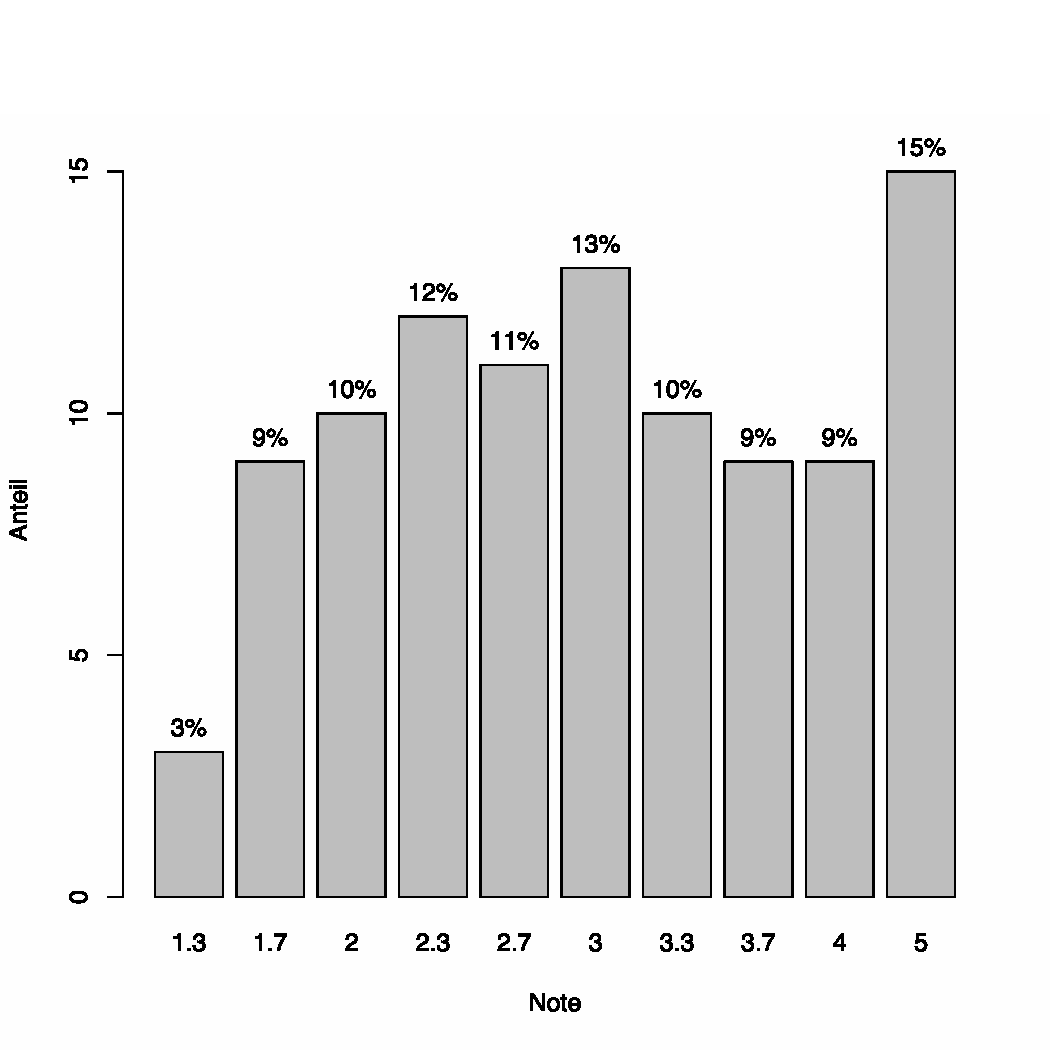
\includegraphics{figures/notenspiegel}}
  \caption{Verteilung der auf akademische Noten umgerechneten Leistungen im Experiment aus \citet{SchaeferSayatz2017a}}
  \label{fig:grammatikkentnissevonstudierenden001}
\end{figure}

Nur 15\% der Teilnehmenden wären durchgefallen, wenn es sich um eine Prüfung gehandelt hätte.
Die restlichen Leistungen verteilen sich nach der Umrechnung auf akademische Noten nahezu gleichmäßig zwischen 1,3 und 4,0.
Solch ein Bild ist vollständig erwartbar, wenn davon ausgegangen wird, dass nicht alle Teilnehmenden dasselbe gelernt haben und die Lernzeitpunkte teilweise sieben Jahre zurückliegen.
Es ist davon auszugehen, dass für jedes andere Schulfach ähnliche Ergebnisse erzielt würden, denn immerhin hatten die Teilnehmenden keine Gelegenheit, sich gezielt auf die gestellten Fragen vorzubereiten.

Allerdings haben, wie oben erwähnt, Studierende aller Bachelor-Semester teilgenommen, und es sollte deshalb eigentlich nicht wundernehmen, wenn das Ergebnis besser als das des bayrischen Eingangstests wäre, bei dem schließlich nur Studierende des ersten Semesters befragt wurden, die noch keine spezifische Ausbildung in germanistischer Linguistik erhalten haben.
Abbildung~\ref{fig:grammatikkentnissevonstudierenden002} schlüsselt die Ergebnisse in Prozent nach Studienjahr auf.

\begin{figure}[htpb]
  \centering
  \resizebox{0.9\textwidth}{!}{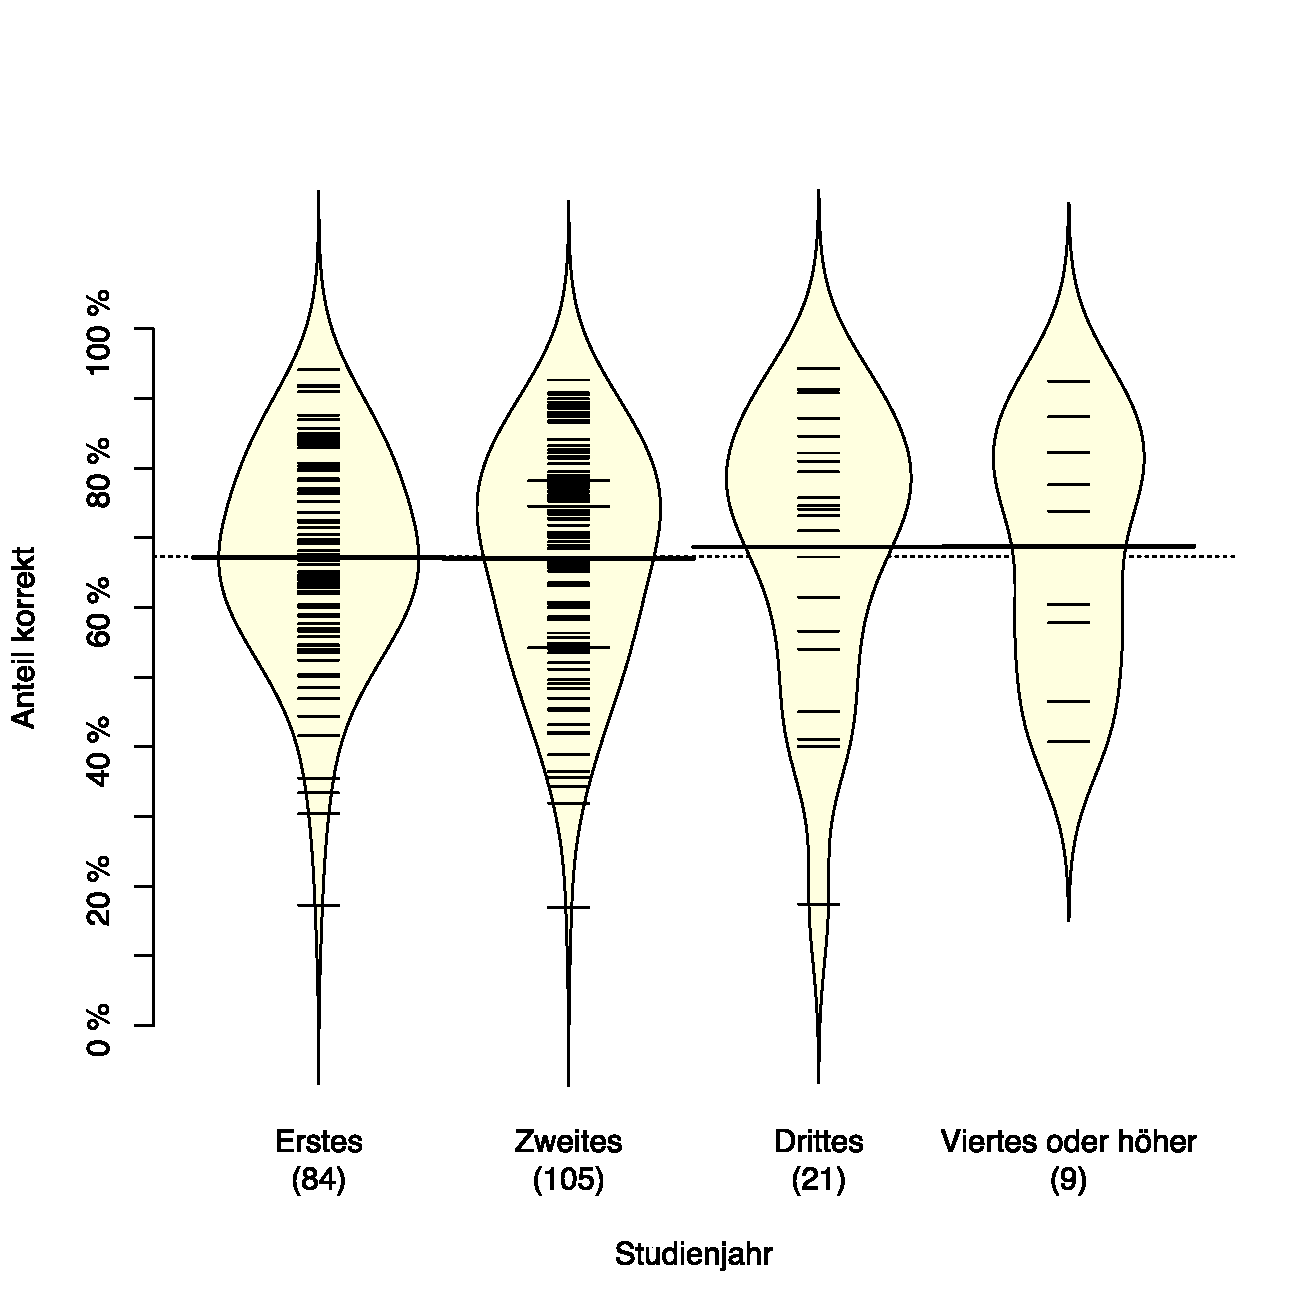
\includegraphics{figures/semester}}
  \caption{Verteilung der erreichten Prozent im Experiment aus \citet{SchaeferSayatz2017a}, gegliedert nach Studienjahr in einem sogenannten Beanplot; jede kurze waagerechte Linie entspricht einem individuellen Ergebnis, die Hüllen entsprechen einer Dichteschätzung der empirischen Verteilung pro Gruppe, die dicken längeren waagerechten Linien markieren den Mittelwert pro Gruppe}
  \label{fig:grammatikkentnissevonstudierenden002}
\end{figure}

\Np

Wie man leicht sieht, werden die Ergebnisse im Verlauf des Studiums im Mittel nicht besser.
Es gibt eine leichte Verschiebung der Verteilung (des Bauchs der jeweiligen Beanplots) nach oben, insbesondere im dritten Studienjahr.
Allerdings wäre schon aufgrund des Ausscheidens leistungs- und motivationsschwächerer Studierender (Fachwechsel oder Studienabbruch) im Laufe der Semester eine stärkere Verbesserung der Leistung zu erwarten.
Wie wir in \citet[242--243]{SchaeferSayatz2017a} argumentieren, kann der Grund der beobachteten Stagnation nicht lokal in der Freien Universität gesucht werden, da sich im Vergleich der Kurrikula mehrerer Universitäten aus verschiedenen Bundesländern zeigt, dass die Freie Universität ein sehr typisches Profil in ihren germanistischen Studiengängen anbietet.

Wir gehen davon aus, dass das Problem vielmehr eine meist nicht optimale Kopplung der universitären Inhalte an die Berufsziele der Studierenden ist.
Wie oben deutlich wurde, sind ca.\ 75\% der Studierenden an der Freien Universität angehende Lehrpersonen, und die Lehre müsste sich deutlich an diesem Berufsziel orientieren.
Von einer anderen Seite nähern sich auch \citet{TopalovicDuenschede2014} demselben Problem.
In einer bundesweiten Umfrage mit 1.019 Lehrpersonen aus allen Schulformen fanden sie im Jahr 2013 heraus, dass sich 48\% der Lehrpersonen durch ihre Ausbildung nicht hinreichend auf den Grammatikunterricht vorbereitet fühlen \citep[76--77]{TopalovicDuenschede2014}.
Dies bestätigt in Form der subjektiven Selbsteinschätzung von Lehrkräften auch unser Ergebnis.

Das Problem ist in seiner Tragweite nicht überzubewerten.
In unserer detaillierten Analyse der besonders problematischen Testfragen haben Ulrike Sayatz und ich herausgefunden, dass Schwierigkeiten vor allem dann auftreten, wenn die Analyse mehr sowohl formale, funktionale und strukturelle Anforderungen an die Studierenden stellt \citep[234--239]{SchaeferSayatz2017a}.
Zum Beispiel werden die syntaktischen Funktionen von Subjekt, Prädikat und Objekt überwiegend richtig zugeordnet, wenn die zu erkennenden Konstituenten in der Aufgabe bereits markiert sind.
Diese Funktionen mussten zum Beispiel den eingeklammerten Konstituenten in Satz (\ref{ex:grammatikkentnissevonstudierenden003}) zugeordnet werden.

\begin{exe}
  \ex\label{ex:grammatikkentnissevonstudierenden003} [Eine Französin] [reiste] [mit ihrem Surfbrett] [über den indischen Ozean].
\end{exe}

Bei dieser Aufgabe wurden im Mittel 84,52\% korrekt gelöst.
Bei einer ähnlichen Aufgabe, bei der allerdings die Konstituenten selber identifiziert werden und dann mit syntaktischen Funktionen analysiert werden sollten, wurden im Mittel nur 51,22\% erreicht.
Ein Beispielsatz ist (\ref{ex:grammatikkentnissevonstudierenden004}).
Die Aufgabe war die Identifikation von Akkusativ- und Dativobjekten.

\begin{exe}
  \ex\label{ex:grammatikkentnissevonstudierenden004} In der Zukunft werden nicht mehr vorwiegend die großen Konzerne die Arbeitsplätze schaffen.
\end{exe}

Abgesehen davon, dass angehende Lehrpersonen im dritten und vierten Studienjahr keinerlei Probleme mit Aufgaben aus dem schulischen Grammatikunterricht mehr haben dürften, zeigen solche Ergebnisse, dass gerade nicht die Fähigkeit ausgebildet wurde, konstruktiv und systematisch mit komplexeren sprachlichen Formen umzugehen.
Unterstrichen wird dies noch dadurch, dass 20,9\% der Teilnehmenden die in (\ref{ex:grammatikkentnissevonstudierenden004}) bebeispielte Aufgabe überhaupt nicht zu lösen versucht haben.
Man kapituliert.
Ergebnisse wie die aus \citet{TopalovicDuenschede2014} und \citet{SchaeferSayatz2017a} sollten als Aufruf an alle Beteiligten verstanden werden, sich intensiver mit dem auseinanderzusetzen, was Lehrende in Schulen in ihrem Beruf zu leisten haben.
Wie \citet[7]{Eisenberg2013c} richtig anmerkt, wird Lehrenden die Grammatik der Lernenden \textit{anvertraut}.
Mit dieser Verantwortung sollten wir nicht fahrlässig umgehen.

In Abschnitt~\ref{sec:studentischesichtweisenaufstudiumundschulunterricht} kommen wir abschließend der Vermutung zuvor, das Problem könnte eine zu niedrige oder eine falsche Motivation von Studierenden sein.


\subsection{Studentische Sichtweisen auf Studium und Schulunterricht}
\label{sec:studentischesichtweisenaufstudiumundschulunterricht}

Im Frühjahr 2018 habe ich eine Umfrage unter Studierenden der Deutschen Philologie an der Freien Universität Berlin durchgeführt.
Die Teilnahme war freiwillig und wurde mittels Google Forms online durchgeführt.
Teilgenommen haben 43 Studierende aus der Bachelor-Phase und eine Studierende aus der Master-Phase.
Das Alter der Teilnehmenden war 21 Jahre im Median und 24,02 Jahre im Mittel.
Vierzig Personen gaben \textit{weiblich} und vier \textit{männlich} als ihr Gender an.%
\footnote{Gender war als Textfeld ohne vorgegebene Optionen ausgelegt.}
Als Hauptfach wurde 18 Mal \textit{Deutsch auf Lehramt}, zwölf Mal \textit{Grundschullehramt} und zwölf Mal \textit{Germanistik (Fachstudium)} angegeben.
Für zwei Teilnehmende war Deutsch das Nebenfach (nicht Lehramt).
Gut 68\% der Teilnehmenden haben also den Lehrberuf als Ziel.

Auf Basis dieser Stichprobe lässt sich nun nicht beliebig verallgemeinern, weil vierzig Teilnehmende die zweite Auflage von \textit{Einführung in die grammatische Beschreibung des Deutschen} verwendet hatten, aber nur vier nicht.
32,5\% der Befragten finden das Buch leicht oder sehr leicht, 52,5\% weder besonders schwer noch besonders leicht, und nur 15\% finden es schwer oder sehr schwer.
75\% finden die didaktische Aufbereitung im Buch gut oder sehr gut, nur 10\% finden sie schlecht oder sehr schlecht.
80\% finden das Buch gut oder sehr gut geeignet als Lektüre im Studium.
Es liegt also die Vermutung nahe, dass sich insbesondere Studierende an der Umfrage beteiligt haben, die gerne mit dem Buch gearbeitet haben, und die das vertretene Konzept von Grammatik befürworten.

Selbst mit dieser Einschränkung sind allerdings einige Ergebnisse relevant.
Eine zentrale Frage war, welche Funktionen der schulische Grammatikunterricht in den Augen der Studierenden haben sollte.%
\footnote{Diese Frage war bis zum Zeitpunkt der Umfrage kein ausführliches Thema von Lehrveranstaltungen.}
Auf Basis von Vortests in Lehrveranstaltungen der letzten Jahre war eine Liste von möglichen Antworten vorgegeben.%
\footnote{Rein formale Punkte wie \textit{Lernen grammatischer Kategorien} wurden dabei durchgehend kritisch gesehen.
Daher wurden sie hier nicht vorgegeben.}
Die Möglichkeit, weitere Antworten frei zu formulieren, wurde daher erwartungsgemäß nur einmal genutzt.
Es konnten bis zu vier Möglichkeiten angekreuzt bzw.\ selber formuliert werden.
Abbildung~\ref{fig:studentischesichtweisenaufstudiumundschulunterricht001} zeigt die prozentuale Verteilung der Antworten.

\begin{figure}[htpb]
  \centering
  \resizebox{0.9\textwidth}{!}{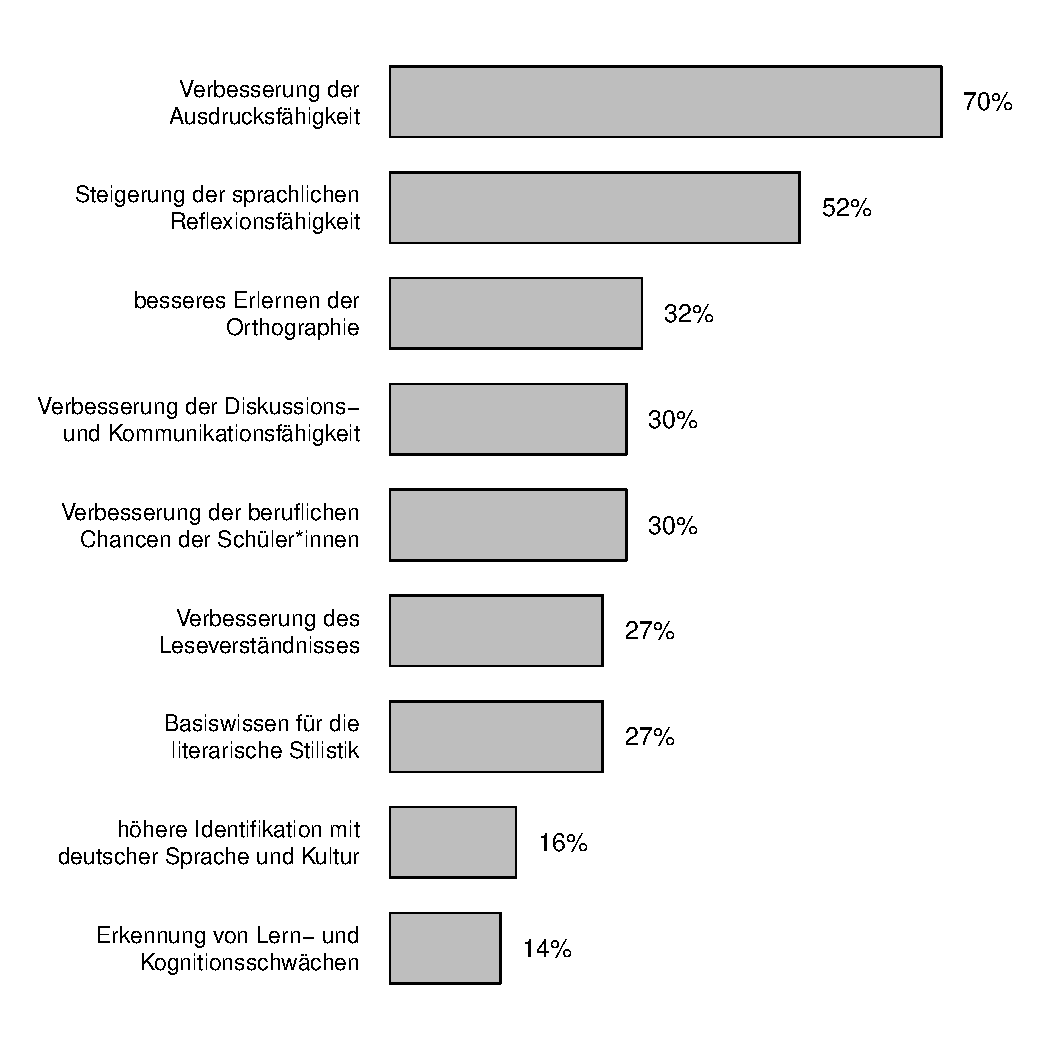
\includegraphics{figures/funktionengrammatikunterricht}}
  \caption{Antworten von Studierenden auf die Frage nach den Funktionen des schulischen Grammatikunterrichts}
  \label{fig:studentischesichtweisenaufstudiumundschulunterricht001}
\end{figure}

Angehende Lehrpersonen sehen also vor allem die Ausbildung in Bildungssprache und Sprachbetrachtung (hier in Form des Begriffs \textit{Reflexionsfähigkeit}) als ihre primären Aufgaben, wenn es um Grammatik in der Schule geht.
Gefragt wurde wohlgemerkt nicht nach der Aufgabe des Deutschunterrichts an sich, sondern spezifisch nach Grammatikunterricht.
Sie sind damit für den hier (vor allem auf Basis von \citealt{Eisenberg2004} und \citealt{Bredel2013}) skizzierten Grammatikunterricht genau richtig eingestellt.

Zudem finden zwar wie oben angemerkt 80\% der Befragten dieses Buch gut oder sehr gut geeignet für ihr eigenes Studium, aber nur 42,5\% finden es gut oder sehr gut als Berufsvorbereitung (30\% schlecht oder sehr schlecht).
Die Ursache kann nur interpretativ gesucht werden.
Entweder sehen Studierende den Praxisbezug nicht direkt genug, worüber gesondert zu diskutieren wäre (sowohl im Sinne einer Verbesserung des Buchs selber als auch einer besseren Erklärung des Zusammenhangs von grammatischem System und schulischer Lehrpraxis).
Außerdem dürfte einigen Befragten bewusst sein, dass eine Betrachtung der Grammatik \textit{alleine} als Berufsvorbereitung nicht ausreicht.
Es müssten also darauf aufbauende Lehrangebote gemacht werden.

Wir haben also gezeigt, dass systematische Grammatik unabdinglich ist für einen erfolgreichen Deutschunterricht, dass daraus spezifische Folgerungen für das Studium gezogen werden können, und dass Studierende durchaus motiviert bei der Sache sind und die Ziele des schulischen Grammatikunterrichts richtig einschätzen.
Gleichzeitig haben wir empirisch (vor allem in Form der Ergebnisse aus \citealt{TopalovicDuenschede2014} und \citealt{SchaeferSayatz2017a}) gezeigt, dass es erhebliche Defizite in der Ausbildung gibt.
\citet[11]{Eisenberg2013c} fordert eine \textit{modellunabhängige} Beschreibung von grammatischen Regularitäten.
Er bemängelt in \citet[13]{Eisenberg2013c}, dass Lehrbücher für das Bachelor-Studium oft von Sprachwissenschaft statt von Sprache handeln, und in \citet[22]{Eisenberg2004}, dass der Linguistik zu viel und der Sprache zu wenig Raum eingeräumt werde.
Das mit diesem Buch vorgelegte Konzept für das Grammatikstudium versteht sich als ein Versuch, diese Mängel zu vermeiden und zu einer Behebung der Defizite beizutragen.

\Zusammenfassung{%
Um Lernende in Sprachbetrachtung auszubilden und ihnen schrift- und bildungssprachliche Kompetenzen zu vermitteln, reicht es nicht aus, dass Lehrpersonen ihre Sprache können.
Vielmehr brauchen sie zusätzlich umfassendes Wissen über diese Sprache, und sie müssen in der Lage sein, Formen und Funktionen dieser Sprache spontan induktiv-konstruktiv zu durchschauen.
Nur mit solchem Wissen und solchen methodischen Fähigkeiten sind Lehrpersonen in einer angemessenen Position, um sprachliche Leistungen zu bewerten, diese Bewertungen zu erklären und sprachliche Probleme von Lernenden zu erkennen und angemessen darauf zu reagieren.
In empirischen Studien zeigt sich allerdings, dass viele Lehrpersonen sich nicht hinreichend auf den Grammatikunterricht vorbereitet fühlen, und dass sie auch nach mehrjährigem Studium nicht unbedingt souverän mit Aufgaben aus real existierenden Grammatik-Schulbüchern umgehen können.
Gleichzeitig sind sie jedoch motiviert (viele sogar hoch motiviert), sich im Studium mit Grammatik zu beschäftigen, und sie schätzen die Aufgaben des schulischen Grammatikunterrichts richtig ein.
Wir haben daher für eine optimale Ausrichtung des Studiums am Bedarf der Mehrheit der Studierenden argumentiert.
}
